\documentclass{article}

\usepackage{hyperref}
\usepackage[dvipsnames]{xcolor}
\usepackage{listings}
\usepackage{amsmath}

\title{Intro to Modern C++ Course Outline}
\author{Ryan Baker}
\date{\today}

\definecolor{JadeGreen}{RGB}{91,158,62}
\lstdefinestyle{catppuccin}{
	backgroundcolor=\color{White},
	commentstyle=\color{Gray},
	numberstyle=\footnotesize\ttfamily\color{Gray},
	stringstyle=\color{JadeGreen},
	keywordstyle=\color{BurntOrange},
	basicstyle=\ttfamily\footnotesize\color{Black},
	breakatwhitespace=false,
	breaklines=true,
	captionpos=b,
	keepspaces=true,
	numbers=left,
	numbersep=5pt,
	showspaces=false,
	showstringspaces=false,
	showtabs=false,
	tabsize=4,
}
\lstset{style=catppuccin}

\hypersetup{
	colorlinks=true,
	hidelinks=false,
	linkcolor=RoyalBlue,
	citecolor=ForestGreen,
	filecolor=DarkOrchid,
	urlcolor=BurntOrange,
	runcolor=BrickRed,
	pdftitle={C++: From Code to Execution},
	pdfauthor={Ryan Baker},
}

\begin{document}

\maketitle
\contentsline{section}{Week \numberline {1:}C++: From Code to Execution
}{}{}
\contentsline{section}{Week \numberline {2:}C++ Control Flow Essentials
}{}{}
\contentsline{section}{Week \numberline {3:}All About Memory
}{}{}
\pagebreak

\centering
\section*{Week 1: C++: From Code to Execution
}	
\documentclass{article}

\usepackage{hyperref}
\usepackage[dvipsnames]{xcolor}
\usepackage{listings}
\usepackage{amsmath}

\title{All About Memory
}
\author{Ryan Baker}
\date{\today}

\definecolor{JadeGreen}{RGB}{91,158,62}
\lstdefinestyle{catppuccin}{
	backgroundcolor=\color{White},
	commentstyle=\color{Gray},
	numberstyle=\footnotesize\ttfamily\color{Gray},
	stringstyle=\color{JadeGreen},
	keywordstyle=\color{BurntOrange},
	basicstyle=\ttfamily\footnotesize\color{Black},
	breakatwhitespace=false,
	breaklines=true,
	captionpos=b,
	keepspaces=true,
	numbers=left,
	numbersep=5pt,
	showspaces=false,
	showstringspaces=false,
	showtabs=false,
	tabsize=4,
}
\lstset{style=catppuccin}

\hypersetup{
	colorlinks=true,
	hidelinks=false,
	linkcolor=RoyalBlue,
	citecolor=ForestGreen,
	filecolor=DarkOrchid,
	urlcolor=BurntOrange,
	runcolor=BrickRed,
	pdftitle={C++: From Code to Execution},
	pdfauthor={Ryan Baker},
}

\begin{document}

\maketitle
\tableofcontents
\pagebreak

\subsection*{Lecture Objectives}

\noindent
By the end of this lecture, you should:
\begin{itemize}
	\item Understand the developer tools needed to write C++
	\item Understand the build process: preprocessing, compilation, linking
	\item Be able to utilize types, arithmetic, and I/O to write a basic C++ program
\end{itemize}

\section{Introduction to C++}

\begin{itemize}
	\item What is C++?
	\begin{itemize}
		\item General-purpose programming language
		\item \textbf{Brief history:} Development, standardization, updates
		\item \textbf{Use cases:} embedded systems, HFT, OS, etc.
	\end{itemize}
	\item Why learn C++?
	\begin{itemize}
		\item There has been a concerted effort to push C++ to the side \begin{itemize}
			\item Some valid concerns (some invalid)
			\item We will investigate throughout the course
		\end{itemize}
		\item Performance, flexibility, power (sharpest tool in the toolbox)
		\item C++ has a very strong ``knowledge passport'' \begin{itemize}
			\item Becoming proficient at C++ is not easy
			\item Proficiency in C++ translates very well to other languages
		\end{itemize}
	\end{itemize}
\end{itemize}

\section{C++ Developer Tools}

\noindent
Two basic tools are needed to develop C++: a \textbf{text editor} and a \textbf{compiler}. You may also use an \textbf{Integrated Development Environment (IDE)} which is a single tool that bundles both.

\subsection{Text Editor}

\begin{itemize}
	\item What is a text editor? A tool to edit text.
	\begin{itemize}
		\item Any tool that lets you edit text is technically workable
	\end{itemize}
	\item Which text editor should I use? \begin{itemize}
		\item \href{https://code.visualstudio.com}{\textbf{Visual Studio Code IDE:}} a beginner-friendly option, very popular
		\item \href{https://www.jetbrains.com/clion/}{\textbf{CLion IDE:}} Premium IDE made by JetBrains, widely appreciated
		\item \textbf{Vim/Nvim:} My choice, steep learning curve, more rewarding \begin{itemize}
			\item Not an IDE, download instructions depend on your OS
			\item Look up ``vim install'' or ``neovim install''
			\item I recommend spending some time configuring your setup, feel free to talk to me for recommendations
		\end{itemize}
	\end{itemize}
\end{itemize}

\subsection{Compiler}

\begin{itemize}
	\item What is a compiler? \begin{itemize}
		\item A compiler is a tool that turns your code into an executable program
		\item Performs lexical analysis, syntax checking, and optimization
	\end{itemize}
	\item Which compiler should I use?
	\begin{itemize}
		\item \textbf{gcc/g++:} One of the best. Download depends on OS
		\item \textbf{clang/llvm:} My personal choice. Download depends on OS
		\begin{itemize}
			\item Best for Mac
		\end{itemize}
		\item \textbf{MSVC:} Microsoft visual compiler, a tier below \textbf{clang} and \textbf{gcc} (IMO)
		\begin{itemize}
			\item An easy option if you're developing on windows
		\end{itemize}
	\end{itemize}
\end{itemize}

\subsection{Hello, World!}

\noindent
With your text editor of choice, write the following code:

\vspace{.5em}
\lstinputlisting[language=C++]{code/helloworld.cpp}
\vspace{.5em}

\noindent
Compile your code using your compiler of choice:

\begin{itemize}
	\item[\texttt{>>}] \texttt{g++ helloworld.cpp -o exe}
	\item[\texttt{>>}] \texttt{clang++ helloworld.cpp -o exe}
\end{itemize}

\noindent
These commands will compile \texttt{helloworld.cpp} and output an executable \texttt{exe}. You can run the executable file:

\begin{verbatim}
	>> ./exe
	Hello, World!
\end{verbatim}

\noindent
The remainder of this lecture will be spent on understanding the process that transforms \texttt{helloworld.cpp} into an executable that prints ``Hello, World!''.

\section{The C++ Build Process}

\noindent
How do we get from the \texttt{.cpp} file to an executable program? Answering this question will allow us to understand and debug our programs more efficiently.

\subsection{Source Code}

\begin{itemize}
	\item \textbf{Source code:} Human-readable code written in \texttt{.cpp} files
	\item $\texttt{main.cpp}\rightarrow\boxed{\textrm{Preprocessor}}\rightarrow\boxed{\textrm{Compiler}}\rightarrow\boxed{\textrm{Linker}}\rightarrow\texttt{main.exe}$
	\item \textbf{Key point:} Source code is just a text file: \begin{itemize}
		\item[\texttt{>>}] \texttt{cp helloworld.cpp ryan.baker}
		\item[\texttt{>>}] \texttt{clang++ -x c++ ryan.baker -o exe \&\& ./exe}
		\begin{itemize}
			\item There is nothing special about \texttt{.cpp} files. The compiler just needs text written in a language called C++.
			\item \texttt{-x} is a flag that clang takes that says: ``The language is C++, even if the file extensions are weird''
		\end{itemize}
	\end{itemize}
\end{itemize}

\subsection{Preprocessor}

\begin{itemize}
	\item What does the preprocessor do? \begin{itemize}
		\item Text substitution: \texttt{\#define MAX 500} replaces ``\texttt{MAX}'' with ``\texttt{500}''
		\item File inclusion: \texttt{\#include <iostream>} copies and pastes \texttt{iostream}
		\begin{itemize}
			\item \texttt{\#include "filename"}: searches current folder, use for local files
			\item \texttt{\#include <filename>}: searches standard include directories
		\end{itemize}
		\item Conditional compilation: \texttt{\#if} and others to select code that compiles
		\end{itemize}
		\vspace{.5em}
		\lstinputlisting[language=C++]{code/preprocessor.cpp}
	\item \textit{Probably won't discuss} \texttt{\#pragma}
	\begin{itemize}
		\item Less relevant in C++ than in C, usually bad practice
	\end{itemize}
	\item Use of \texttt{-E} to view preprocessor output \begin{itemize}
		\item[\texttt{>>}] \texttt{clang++ -E preprocessor.cpp > preprocessor\_output.cpp} \begin{itemize}
			\item \texttt{iostream} file has been copied and pasted in
			\item macros \texttt{MAX} and \texttt{STATUS} have been expanded to their values
		\end{itemize}
	\end{itemize}
	\item \textbf{Key point:} \texttt{preprocessor\_output.cpp} is the same as \texttt{preprocessor.cpp} \begin{itemize}
		\item[\texttt{>>}] \texttt{clang++ preprocessor\_output.cpp -o exe \&\& ./exe}
		\begin{itemize}
			\item This command produces the same thing as the first program
		\end{itemize}
	\end{itemize}
\end{itemize}

\subsection{Compiler}

\begin{itemize}
	\item What does the compiler do? \begin{itemize}
		\item Reads the output of the preprocessor and turns it to machine code
		\item Responsible for alerting the user about various types of errors
		\item Outputs object files (\texttt{.o} or \texttt{.obj}) \begin{itemize}
			\item Mostly machine code, has some directives for the linker to use
		\end{itemize}
	\end{itemize}
	\item Use of \texttt{-c} to view the object file (completely unreadable)\begin{itemize}
		\item \texttt{-c} stands for ``just compile'' (don't link)
		\item[\texttt{>>}] \texttt{clang++ -c helloworld.cpp} produces \texttt{helloworld.o}
		\item[\texttt{>>}] \texttt{clang++ helloworld.o -o exe \&\& ./exe} runs the program
	\end{itemize}
	\item Use of \texttt{-S} to view the assembly output (readable)\begin{itemize}
		\item[\texttt{>>}] \texttt{clang++ -S helloworld.cpp} produces \texttt{helloworld.s}
		\item Contains traces of our original program
		\item[\texttt{>>}] \texttt{clang++ helloworld.s -o exe \&\& ./exe} runs the program
	\end{itemize}
\end{itemize}

\subsection{Linker}

\begin{itemize}
	\item What does the linker do? \begin{itemize}
		\item Resolves symbols, matching declarations to definitions
		\item Combines multiple translation units into an executable
		\item This allows us to write code across files, enhancing modularity
	\end{itemize}
	
	\lstinputlisting[language=C++]{code/file2.hpp}
	\lstinputlisting[language=C++]{code/file1.cpp}
	\lstinputlisting[language=C++]{code/file2.cpp}

	\item \textbf{Key point:} \texttt{clang++ file1.cpp -o exe} produces a linker error \begin{itemize}
		\item The symbol ``\texttt{greet()}'' is not defined
		\item Recognize the difference between compilation and linking errors \begin{itemize}
			\item Linker errors are often more convoluted
			\item Often denoted by ``\texttt{ld:}'' or ``\texttt{linker error:}'' 
		\end{itemize}
	\end{itemize}
	\item[\texttt{>>}] \texttt{clang++ file1.cpp file2.cpp -o exe} \begin{itemize}
		\item We need to pass in \texttt{file2.cpp} to the linker
	\end{itemize}
\end{itemize}

\section{C++ Programming Basics}

\subsection{Types and Variables}

\noindent
All programming involves storing and manipulating data, typically in variables. A variable's \textit{datatype} defines the set of values it can hold. For example, a \texttt{char}acter datatype represents letters like `a' through `z', while a \texttt{bool}ean datatype represents true or false.

\vspace{1em}	
\noindent
C++ has some built-in datatypes, called \textit{primitive} or \textit{integral} datatypes. Each datatype is designed to serve a different purpose. However, with a low-level programming language such as C++, \textbf{the only real difference} between any of these datatypes is \textbf{the amount of memory} they occupy.

\begin{itemize}
	\item \texttt{int}: represents an integer
		\begin{itemize}
			\item[\texttt{>>}] \texttt{int x = 42;} assigns the value 42 to a variable `x'
			\item[\texttt{>>}] \texttt{sizeof(x); sizeof(int)} returns the \# of bytes `x' occupies
			\item Because `x' occupies a finite number of bytes, its range is limited
			\begin{itemize}
				\item We can calculate its total range as $2^w$ where $w$ represents the width of `x' in bits
				\item Note that the maximum value may be halved if `x' is signed
			\end{itemize}
			\item If we want a smaller int, we use \texttt{short}. If we want a longer int, we can use \texttt{long} or \texttt{long long}
			\begin{itemize}
				\item I find these names very confusing
				\item I recommend \texttt{\#include <cstdint>}
			\end{itemize}
			\item Signedness: we can prepend a `u` or \texttt{unsigned} to the type to make the number unsigned. This expands its positive range
		\end{itemize}
		\item \texttt{char}: represents a character
		\begin{itemize}
			\item[\texttt{>>}] \texttt{char letter = `a';} assigns `a' to `letter'
				\begin{itemize}
					\item \texttt{`a'} is really just a number
					\item[\texttt{>>}] \texttt{int x = `a'; std::cout << x << std::endl;}
				\end{itemize}
		\end{itemize}
		\item \texttt{float}, \texttt{double}: represents a floating-point (fractional) type
		\begin{itemize}
			\item \texttt{double} is (usually) twice as large as a \texttt{float}
			\item \texttt{sizeof(double)} = 8, \texttt{sizeof(float)} = 4 (usually)
		\end{itemize}
		\item \texttt{bool}: represents a boolean value (True or False)
		\begin{itemize}
			\item \texttt{sizeof(bool)} = 1 (usually)
		\end{itemize}
		\item \texttt{void}: represents ``no type''
		\begin{itemize}
			\item \texttt{sizeof(void)} is a senseless operation, produces an error
	\end{itemize}
\end{itemize}

\subsection{Input and Output with \texttt{iostream}}

\noindent
Our programs are useless unless we can communicate with them. C++ provides various methods of passing data into and out-of our programs. The \texttt{iostream} library is the most widely used library for input and printing data in C++.

\begin{itemize}
	\item ``\texttt{iostream}'' stands for input and output (IO) stream
	\begin{itemize}
		\item[\texttt{>>}] \texttt{\#include <iostream>}
	\end{itemize}
	\item Output with \texttt{iostream}
	\begin{itemize}
		\item \texttt{std::cout} is used to print data to the console
		\begin{itemize}
			\item \texttt{std::} is a namespace access, says search namespace ``\texttt{std}'' (standard) for function called ``\texttt{cout}''
			\item We will discuss namespaces later in the course
		\end{itemize}
		\item \texttt{std::endl} is used to output a newline and flush the buffer
		\item The `\texttt{<<}' operator is the output stream operator
	\end{itemize}
	\item Input with \texttt{iostream}
	\begin{itemize}
		\item \texttt{std::cin} is used to fetch data at runtime from the user
		\item The `\texttt{>>}' operator is the stream input operator
	\end{itemize}
\end{itemize}

\noindent
We will discuss the workings of \texttt{iostream} more in depth when we discuss \textbf{streams}. Presently, just get familiar with the syntax of \texttt{cin} and \texttt{cout}.

\vspace{.5em}
\lstinputlisting[language=C++]{code/iostreamio.cpp}

\end{document}

\centering
\section*{Week 2: C++ Control Flow Essentials
}	
\documentclass{article}

\newcommand{\titleone}{Introduction and Setup}
\newcommand{\titletwo}{C++ Programming Basics}
\newcommand{\titlethree}{How C++ Works}
\newcommand{\titlefour}{Introduction to OOP}
\newcommand{\titlefive}{Advanced OOP}
\newcommand{\titlesix}{Templates}
\newcommand{\titleseven}{The C++ Standard Library}
\newcommand{\titleeight}{Safety in C++}
\newcommand{\titlenine}{Compile-Time Programming}

\newcommand{\thistitle}{\titletwo}
\newcommand{\me}{Ryan Baker}

\usepackage{hyperref}
\usepackage[dvipsnames]{xcolor}
\usepackage{listings}

\title{\thistitle}
\author{\me}
\date{\today}

\definecolor{JadeGreen}{RGB}{91,158,62}
\lstdefinestyle{catppuccin}{
	backgroundcolor=\color{White},
    commentstyle=\color{CadetBlue},
	numberstyle=\footnotesize\ttfamily\color{Gray},
	stringstyle=\color{JadeGreen},
	keywordstyle=\color{BurntOrange},
	basicstyle=\ttfamily\color{Black},
	breakatwhitespace=true,
	breaklines=true,
	captionpos=b,
	keepspaces=true,
	numbers=left,
	numbersep=5pt,
	showspaces=false,
	showstringspaces=false,
	showtabs=false,
	tabsize=4,
}

\lstset{style=catppuccin}

\hypersetup{
	colorlinks=true,
	hidelinks=false,
	linkcolor=RoyalBlue,
	citecolor=ForestGreen,
	filecolor=DarkOrchid,
	urlcolor=BurntOrange,
	runcolor=BrickRed,
    pdftitle={\thistitle},
	pdfauthor={\me},
}

\newcommand{\inlinecpp}[1]{\lstinline[language=C++]|#1|}
\newcommand{\centercpp}[1]{\begin{center}\lstinline[language=C++]|#1|\end{center}}
\newcommand{\inputcpp}[1]{\lstinputlisting[language=C++]{#1}}


\title{\thistitle}
\author{\me}
\date{\today}

\begin{document}

\maketitle
\tableofcontents
\pagebreak

\section{The Build Process}

\subsection{Source Code}

\subsection{Preprocessor}

\subsubsection{Text Substitution}

\subsubsection{Conditional Compilation}

\subsubsection{File Inclusion}

\subsubsection{Preprocessor Output}

\subsection{Compilation}

\subsubsection{Compiler Output}

\subsection{Linking}

\section{Introduction to Memory}

\subsection{How C++ Uses Memory}

\subsection{Pointers}

\subsubsection{\inlinecpp{NULL} Pointers}

\subsubsection{Pointer Arithmetic}

\subsubsection{Pointers to Pointers}

\section{Memory Layout}

\subsection{Text Segment}

\subsection{Static Memory}

\subsubsection{Variable Lifetime}

\subsection{The Heap}

\subsubsection{Operators \inlinecpp{new} and \inlinecpp{delete}}

\subsubsection{Memory Leaks}

\subsection{The Stack}

\subsubsection{The Stack Pointer}

\end{document}


\centering
\section*{Week 3: All About Memory
}	
\documentclass{article}

\usepackage{hyperref}
\usepackage[dvipsnames]{xcolor}
\usepackage{listings}
\usepackage{amsmath}
\usepackage{tikz}

\title{All About Memory
}
\author{Ryan Baker}
\date{\today}

\definecolor{JadeGreen}{RGB}{91,158,62}
\lstdefinestyle{catppuccin}{
	backgroundcolor=\color{White},
	commentstyle=\color{Gray},
	numberstyle=\footnotesize\ttfamily\color{Gray},
	stringstyle=\color{JadeGreen},
	keywordstyle=\color{BurntOrange},
	basicstyle=\ttfamily\footnotesize\color{Black},
	breakatwhitespace=false,
	breaklines=true,
	captionpos=b,
	keepspaces=true,
	numbers=left,
	numbersep=5pt,
	showspaces=false,
	showstringspaces=false,
	showtabs=false,
	tabsize=4,
}
\lstset{style=catppuccin}

\hypersetup{
	colorlinks=true,
	hidelinks=false,
	linkcolor=RoyalBlue,
	citecolor=ForestGreen,
	filecolor=DarkOrchid,
	urlcolor=BurntOrange,
	runcolor=BrickRed,
	pdftitle={C++: From Code to Execution},
	pdfauthor={Ryan Baker},
}

\begin{document}

\maketitle
\tableofcontents
\pagebreak

\subsection*{Lecture Objectives}

\noindent By the end of this lecture, you should:
\begin{itemize}
	\item Understand pointers, references, and indirection
	\item Be able to use arrays to store and manipulate many variables
	\item Be able to reason about memory segments, and how they effect execution
\end{itemize}

\section{Pointers}

\noindent
Computers work with memory. Everything, from variables, to functions, to the actual machine code itself is stored in memory. Memory is extremely important. Pointers are tools to accessing and manipulating memory.

\subsection{Basics of Pointers}

\begin{itemize}
	\item What is a pointer?
	\begin{itemize}
		\item A pointer is a variable (an integer) that represents a memory address
	\end{itemize}
	\item Why use pointers? Pointer provide:
	\begin{itemize}
		\item Dynamic memory allocation and deallocation
		\item Passing large objects efficiently to functions
		\item Manipulation of memory at a low-level
	\end{itemize}
	\item Pointer syntax: \texttt{<type>* <name>}
	\begin{itemize}
		\item \textbf{Example:} \texttt{int* ptr;} declares a pointer to an \texttt{int}
		\item \textbf{Example:} \texttt{int* ptr = nullptr;} declares a \texttt{NULL} pointer to an \texttt{int}
		\begin{itemize}
			\item \texttt{nullptr} is a keyword that represents a null pointer value
			\item \texttt{NULL} is a pointer value that points to address 0 (invalid)
		\end{itemize}
	\end{itemize}
	\item Using pointers:
	\begin{itemize}
		\item Address-of operator: \texttt{\&}
		\begin{itemize}
			\item Use the address-of operator in front of a variable to get its address
			\item \texttt{std::cout << \&x << std::endl;} prints the address of \texttt{x}
			\item \texttt{int* ptr = \&x;} sets the value of \texttt{ptr} to the address of \texttt{x}
		\end{itemize}
		\item Dereference operator: \texttt{*}
		\begin{itemize}
			\item Use the dereference operator in front of a pointer to get the value
			\item \texttt{std::cout << *ptr << std::endl;} prints the value pointed to
			\item \texttt{int x = *ptr;} sets the value of \texttt{x} to the the memory pointed to by \texttt{ptr}
		\end{itemize}
		\item Together, the address-of and dereference operators allow you to access and manipulate memory with pointers
	\end{itemize}
\end{itemize}

\lstinputlisting[language=C++]{code/pointer.cpp}

\subsection{Pointer Arithmetic}

\begin{itemize}
	\item What is pointer arithmetic?
	\begin{itemize}
		\item Pointer arithmetic involves performing operations (such as addition or subtraction) on pointer variables, adjusting the memory address they reference based on the size of the data type they point to.
	\end{itemize}
	\item Pointer arithmetic in action:
	\lstinputlisting[language=C++]{code/parithmetic.cpp}
	\item \textbf{Key point:} Pointer arithmetic on \texttt{void*}s causes errors because \texttt{sizeof(void)} is undefined
\end{itemize}

\subsection{Pointers to Pointers}

\begin{itemize}
	\item Pointers are variables that represent memory addresses of other variables
	\item This means that a pointer can ``point to'' another pointer
	\begin{itemize}
		\item \texttt{sizeof(<pointer>)} = 8 (usually, for 64-bit systems)
		\begin{itemize}
			\item If you're working on a 32-bit system: \texttt{sizeof(<pointer>)} = 4
		\end{itemize}
	\end{itemize}
	\lstinputlisting[language=C++]{code/ptop.cpp}
\end{itemize}

\section{References}

\noindent
Every reference is just a pointer in disguise. They exist to help make working with pointers a bit easier.

\begin{itemize}
	\item What is a reference?
	\begin{itemize}
		\item A reference is a way to ``reference'' an existing variable
		\item There is no such thing as a \texttt{NULL} reference
		\item Think of references as aliases
	\end{itemize}
	\item Reference syntax: \texttt{<type>\& <name> = <variable>}
	\begin{itemize}
		\item \textbf{Example:} \texttt{int\& ref = x;} ``refers'' \texttt{ref} to \texttt{x}
	\end{itemize}
	\lstinputlisting[language=C++]{code/reference.cpp}
	\item\textbf{Example:} \texttt{increment(int x) \{...\}} vs. \texttt{increment(int\& x) \{...\}}
	\begin{itemize}
		\item When you pass by reference, the original value is modified
		\item When you pass by value (not reference), the original is untouched
	\end{itemize}
\end{itemize}

\section{Arrays}

\begin{itemize}
	\item What is an array?
	\begin{itemize}
		\item An array is a collection of variables stored contiguously
		\item Truly, an array is simply a pointer to its first element
	\end{itemize}
	\item When to use arrays?
	\begin{itemize}
		\item We often need to represent an entire collection of data, rather than creating many many variables, we can create an array
		\item \textbf{Example:} To represent the squares of a chess board, I could either create 64 variables: \texttt{int a1, int b1, ... int h8}, or use an array
	\end{itemize}
	\item Array syntax: \texttt{<type> <name>[<size>] = \{...\}}
	\begin{itemize}
		\item \textbf{Example:} \texttt{int chess\_board[64];}
	\end{itemize}
	\item Using arrays: \texttt{<name>[<index>]}
	\begin{itemize}
		\item Indices start at 0
		\item \textbf{Example:} \texttt{int square = chess\_board[32];}
		\item The square bracket (access) operator \texttt{[]} expands to a dereference:
		\begin{itemize}
			\item \texttt{arr[5]} $\rightarrow$ \texttt{*(arr + 5)} (Recall pointer arithmetic)
			\item This is why indices begin at 0
			\item To prove this: \texttt{arr[5] == 5[arr]}
		\end{itemize}
	\end{itemize}
	\lstinputlisting[language=c++]{code/access.cpp}
\end{itemize}

\section{Memory Segments}

\noindent
The memory that your operating system assigns to your executable is split up into different segments. Each segment is designed to hold a different type of data.

\begin{center}
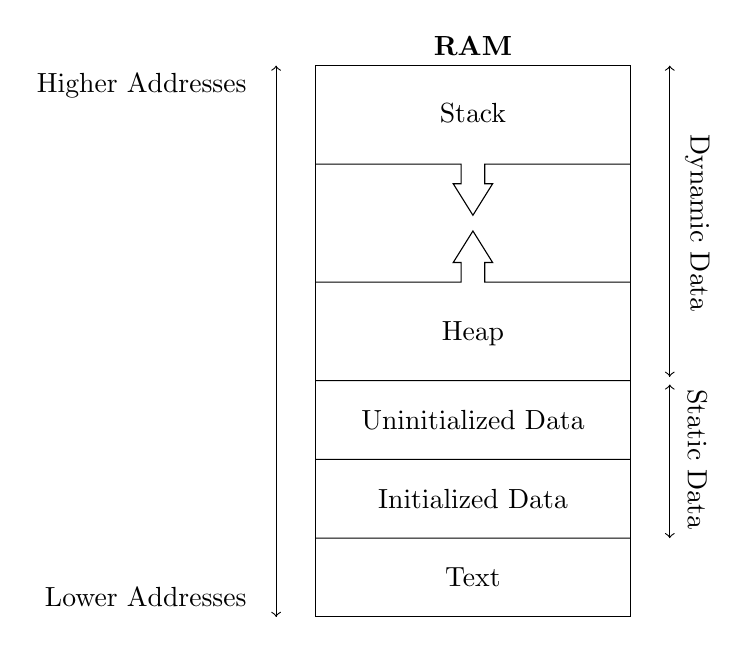
\begin{tikzpicture}

\draw
(0,0) -- ++(4,0) -- ++(0,7) -- ++(-4,0) -- (0,0)
;
\draw[->](-0.5,0) -- (-0.5,7);
\draw[->](-0.5,7) -- (-0.5,0);
\draw
(-0.75,6.75) node[left] {Higher Addresses}
(-0.75,0.25) node[left] {Lower Addresses}
(2,7) node[above] {\textbf{RAM}}
(0,1) -- (4,1) (2,0.5) node[] {Text}
(0,2) -- (4,2) (2,1.5) node[] {Initialized Data}
(0,3) -- (4,3) (2,2.5) node[] {Uninitialized Data}
(0,4.25) -- ++(1.85,0) -- ++(0,0.25) -- ++(-0.1,0) -- ++ (0.25,0.4) -- ++(0.25,-0.4) -- ++(-0.1,0) -- ++(0,-0.25) -- ++(1.85,0)
(0,5.75) -- ++(1.85,0) -- ++(0,-0.25) -- ++(-0.1,0) -- ++ (0.25,-0.4) -- ++(0.25,0.4) -- ++(-0.1,0) -- ++(0,0.25) -- ++(1.85,0)
(2,3.6) node[] {Heap}
(2,6.4) node[] {Stack}
;
\draw[->] (4.5,1)--(4.5,2.95) ;
\draw[->] (4.5,2.95)--(4.5,1) ;
\draw[->] (4.5,3.05) --(4.5,7);
\draw[->] (4.5,7) --(4.5,3.05);
\draw
(4.85,5) node[rotate=-90] {Dynamic Data}
(4.85,2) node[rotate=-90] {Static Data}
;
\end{tikzpicture}
\end{center}

\subsection{Text Segment}

\noindent
The text segment, a.k.a. the ``code'' segment, contains the machine code instructions to run your program. It is fixed in size and read-only. It also contains integer and string literals present in your code.

\subsection{Static Memory}

\noindent
Static memory is allocated at compile time and read directly from the executable. It contains global and static variables. This segment is divided into \textit{initialized} and \textit{uninitialized} data. The only difference is whether or not the variable has a compile-time initialized value.

\subsection{Heap Memory}

\begin{itemize}
	\item What is the heap?
	\begin{itemize}
		\item The heap is a memory segment that is variable in size and used for dynamic memory allocation.
        \item It gives the programmer direct control over memory, allowing you to allocate and deallocate memory manually.
        \item Think of it as a large pool of memory available for your program's use (though the term ``heap'' doesn't refer to this).
	\end{itemize}
	\item How to use the heap?
	\begin{itemize}
		\item Use the \texttt{new} operator to allocate memory:
		\begin{itemize}
		\item \texttt{int* ptr = new int(42);} Allocates an \texttt{int} with value 42
		\end{itemize}
		\item Use the \texttt{delete} operator to free memory:
		\begin{itemize}
		\item \texttt{delete ptr;} Frees the memory allocated to \texttt{ptr}
		\end{itemize}
	\end{itemize}
	\lstinputlisting[language=C++]{code/heap.cpp}
	\item \textbf{Memory leaks:}
	\begin{itemize}
		\item A memory leak occurs when memory is allocated on the heap but never freed, causing the program to consume more memory over time.
		\item Forgetting to deallocate memory with \texttt{delete} leads to memory leaks
		\item Dereferencing pointers that have been deleted is undefined behavior
		\item In short, manual memory management is somewhat error prone, especially in large or collaborative projects.
		\item Modern C++ provides alternatives to \texttt{new} and \texttt{delete} (covered in the future)
	\end{itemize}
	\lstinputlisting[language=C++]{code/leak.cpp}
\end{itemize}

\subsection{Stack Memory}

\noindent
The stack is where local variables and function arguments live. The name ``stack'' refers to how the structure operates. It works like a stack of books, where the last one placed down is the first one popped off.

\vspace{1em}
\noindent
Every time a new function is called, a stack frame is pushed onto the stack. This stack frame contains the function's arguments and local variables. You may only ever directly access the top stack frame, hence scoped variables. When the function returns, its stack frame is popped off the top.

\end{document}


\end{document}
